\documentclass{spbau-diploma}

% пакеты
\usepackage{amsthm}
\usepackage{amssymb}
% \usepackage{mdsymbol}
\usepackage{mathtools}
\usepackage{algorithm}
\usepackage[singlelinecheck=false,justification=justified]{caption}
\usepackage{algorithmicx}
\usepackage[noend]{algpseudocode}
\usepackage{tikz}
\usetikzlibrary{fit,automata,positioning}
\usetikzlibrary{decorations.pathmorphing}
\tikzset{
  snake it/.style={decorate, decoration=snake},
  every state/.style={minimum size=0.3cm}}

\usepackage{perpage}
\MakePerPage{footnote}
% \renewcommand{\thefootnote}{\fnsymbol{footnote}}

% Основные математические символы
\def\eps{\varepsilon}                  % eps
\def\oo{\infty}                        % oo
\def\SO{\Rightarrow}                   % =>
\def\EQ{\Leftrightarrow}               % <=>
\def\t{\texttt}                        % mono font
\def\s{\textsc}                        % small capitals (for problem names)
\def\c#1{{\rm\sc{#1}}}                 % font for classes \t{NP} etc
\def\O{\mathcal{O}}                    % cool big O
\def\NO{\t{\#}}                        % #
\def\edge{\leftrightarrow}             % <->
\def\to{\rightarrow}                   % ->
\def\path{\rightsquigarrow}            % ~~>
\def\su{\sum\limits}                   % sum
\renewcommand{\le}{\leqslant}          % <=, beauty
\renewcommand{\ge}{\geqslant}          % >=, beauty
\newcommand{\q}[1]{\langle #1 \rangle} % <x>
\newcommand{\cool}[1]{\mathcal{#1}}    % fancy letters

\def\TODO{{\color{red}{\bf TODO}}}

\newtheorem{theorem}{Теорема}[section]
\newtheorem{lemma}{Лемма}[section]
\newtheorem{example}{Пример}[section]
\newtheorem{proposition}{Утверждение}[section]
\newtheorem{corollary}{Следствие}[theorem]

\theoremstyle{remark}
\newtheorem*{remark}{Замечание}
\newtheorem*{note}{Замечание}

\theoremstyle{definition}
\newtheorem{definition}{Определение}[section]

\begin{document}
% Год, город, название университета и факультета предопределены,
% но можно и поменять.
% Если англоязычная титульная страница не нужна, то ее можно просто удалить.
\filltitle{ru}{
    chair              = {Кафедра математических и информационных технологий},
    title              = {Пустое подмножество как замкнутое множество},
    % Здесь указывается тип работы. Возможные значения:
    %   coursework - Курсовая работа
    %   diploma - Диплом специалиста
    %   master - Диплом магистра
    %   bachelor - Диплом бакалавра
    type               = {master},
    position           = {студента},
    group              = 666,
    author             = {Машкин Эдельвейс Захарович},
    supervisorPosition = {д.\,ф.-м.\,н., профессор},
    supervisor         = {Выбегалло А.\,А.},
    reviewerPosition   = {ст. преп.},
    reviewer           = {Привалов А.\,И.},
    chairHeadPosition  = {д.\,ф.-м.\,н., профессор},
    chairHead          = {Омельченко А.\,В.},
    % university = {САНКТ-ПЕТЕРБУРГСКИЙ АКАДЕМИЧЕСКИЙ УНИВЕРСИТЕТ},
    % faculty = {Центр высшего образования},
    % city = {Санкт-Петербург},
    % year             = {2013}
}
\filltitle{en}{
    chair              = {Department of Mathematics and Information Technology},
    title              = {Empty subset as closed set},
    author             = {Edelweis Mashkin},
    supervisorPosition = {professor},
    supervisor         = {Amvrosy Vibegallo},
    reviewerPosition   = {assistant},
    reviewer           = {Alexander Privalov},
    chairHeadPosition  = {professor},
    chairHead          = {Alexander Omelchenko},
}
\maketitle
\tableofcontents

% \section*{Аннотация}

Аннотируем

\pagebreak

Very abstract
% У введения нет номера главы
\section*{Введение}

% Задача поиска путей с контекстно-свободными ограничениями была сформулирована \cite{Yannakakis1990} Михалисом Янакакисом в 1990 году в терминах запросов к графовым базам данных. С тех 

\subsection*{Актуальность}

Графовые модели данных широко используются в различных областях, например, в биоинформатике~\cite{Sevon08}, анализе социальных сетей~\cite{Zarrinkalam14, Chaudhary16}, графовых базах данных~\cite{Medeiros18,Yannakakis1990} и разных видах статического анализа (\TODO: ссылки). 

Одной из важных задач в анализе графовых моделей данных является поиск путей с заданными ограничениями. Одним из способов задавать такие ограничения являются формальные языки: если на рёбрах графа написаны метки из фиксированного алфавита, то можно искать пути, конкатенация меток на которых принадлежит фиксированному языку~\cite{Barrett00}. Например, хорошо изучена задача поиска путей с ограничениями, заданными регулярными языками (\TODO: link). В этой же работе мы остановимся на классе контекстно-свободных языков (\TODO: link (?)), так как они позволяют решать более широкий класс задач.

Задача поиска путей с контекстно-свободными ограничениями, или, сокращённо, CFPQ\footnote{Context-Free Path Querying} была сформулирована Михалисом Яннакакисом в 1990 году~\cite{Yannakakis1990} в применении к запросам к декларативному языку Datalog~\cite{DatalogWiki, Ceri1989}. С тех пор было предложение множество алгоритмов для её решения, в основном, основанных на разных видах синтаксического анализа: алгоритм Репса~\cite{Reps97}, использующий метод, схожий с алгоритмом Кока-Янгера-Касами~\cite{Younger1967},
 алгоритм Хеллингса~\cite{Hellings15}, использующий аннотированные грамматики и другие~\cite{Santos18,Azimov18, Medeiros18, Orachev20, Chaudhuri08}. 

 К сожалению, недавно Кёйперс и др. экспериментально показали~\cite{Kuijpers19}, что текущие методы не достаточно эффективны для использования на практике. Что не удивительно, так как все они имеют асимптотику $\O(n^3)$ (где $n$~--- размер входного графа, а размер грамматики~--- константа), и лучшее ускорение, которого можно добиться, уменьшает время работы лишь в $\O(\log n)$ раз~\cite{Chaudhuri06} (используя метод четырёх русских~\cite{Arlazarov70}). Более того, существует условная нижняя оценка~\cite{Heintze1997,Chatterjee17}, согласно которой не существует комбинаторного\footnote{Этот термин не вполне определен, но можно понимать его как ``не алгебраический''. В частности, комбинаторные алгоритмы не должны использовать деление и вычитание, так те пользуются особенностями алгебраических структур (а именно, существованием обратного)} субкубического\footnote{С временем работы $\O(n^{3 - \eps})$} алгоритма для задачи CFPQ.

 Всё вышесказанное приводит к тому, что имеет смысл разрабатывать алгоритмы для частных случаев задачи, имеющие лучшее время работы. 

 Данная работа нацелена 

\subsection*{Постановка задачи и ключевые термины}

\TODO: \textit{Может, это подвинуть в Literature review?}

Для формальной постановки задачи потребуется ввести некоторые вспомогательные определения.

\begin{definition}
% [Помеченный граф]
    \textit{Ориентированный помеченный граф} (или граф с метками)~--- это тройка $G = \langle V, E, \Sigma \rangle$, где $V$~--- множество вершин, $\Sigma$~--- множество меток, $E \subseteq V \times V \times \Sigma$~--- множество рёбер. 

    Неформально, это обычный мультиграф, каждому ребру которого сопоставлена метка из алфавита $\Sigma$.
\end{definition}

\begin{definition}
% [Контекстно-свободная грамматика]
\textit{Контекстно-свободная грамматика}~--- это четвёрка $\langle \Sigma, N, S, P \rangle$, где
\begin{itemize}
    \item $\Sigma$~--- конечный алфавит
    \item $N$~--- конечное множество нетерминалов
    \item $S \in N$~--- стартовый нетерминал
    \item $P$~--- конечное множество продукций (правил грамматики), имеющих вид\\ $N_i \to \alpha$, где $N_i \in N, \alpha \in (\Sigma \cup N)^{*}$
\end{itemize}
\end{definition}

\begin{example}
\TODO: пример
\end{example}


\begin{definition}
% [Контекстно-свободный язык]
\textit{Контекстно-свободный язык}~--- это язык, распознаваемый контекстно-свободной грамматикой

\end{definition}

Теперь определим саму задачу.

\begin{definition}
% [Задача поиска путей с контекстно-свободными ограничениями]
    Входной граф: $G$

    Входная грамматика: $\cool{G}$

    РКА входной грамматики: $\cool{R}$

    % Написать про семантику: https://arxiv.org/pdf/1502.02242.pdf

\end{definition}

Теперь будут введены некоторые понятие (в основном, из теории формальных языков), которые встретятся далее по тексту работы.

\begin{definition}[Язык Дика]
    Языком Дика на $k$ типах скобок $(D_k)$ называют контекстно-свободный язык над алфавитом $\Sigma_k = \{ (_1, )_1, (_2, )_2 \dots (_k, )_k \}$, состоящий из правильных скобочных последовательностей на $k$ типах скобок.

    Задачу CFPQ для языка Дика называют также задачу Диковой достижимости (Dyck-reachability).
\end{definition}

\begin{definition}[Двунаправленный граф]
    Помеченный граф $G = \langle V, E, \Sigma_k \rangle$ называется двунаправленным (bidirected), если в нём для каждого ребра $\langle u, v, (_i \rangle$ найдётся противоположное ребро $\langle v, u, )_i \rangle$ и наоборот.

    Неформально, матрица смежности такого графа симметрична, и метки на симметричных рёбрах~--- это парные открывающая/закрывающая скобки.
\end{definition}

\begin{definition}[Система Непересекающихся Множеств (СНМ)]

\end{definition}

\subsection*{Цель и задачи}

% \subsection*{Достигнутые результаты}

% Какие результаты, я же ничего не делала весь год..

\subsection*{Структура работы}
\section{Обзор литературы}

\section{Ключевые понятия и термины}

\TODO: нет такой главы, это всё по другим главам расползётся

\subsection{Основные понятия из теории формальных языков}



\begin{definition}[Конечный автомат (?)]
    НКА и ДКА
    
\end{definition}

\begin{definition}[Рекурсивный конечный автомат (РКА)]
    \textit{Для простоты тут будет немного не такое определение, как в~\cite{Alur05}}

    Это набор компонент $M_1, M_2, \dots , M_k$, где каждая компонента $M_i$~--- это пятёрка $\langle Q_i, \Sigma_i, En_i, Ex_1, \delta_i \rangle$, где 
        \begin{itemize}
          \setlength\itemsep{-0.1em}
          \item $Q_i$~--- конечное множество состояний
          \item $\Sigma_i$~--- конечный алфавит
          \item $En_i \subset Q_i$~--- множество начальных состояний
          \item $Ex_i \subset Q_i$~--- множество конечных состояний
          \item $\delta_i \colon Q_i \times (\Sigma_i \cup \bigcup\limits_{j = 1}^k En_i \times Ex_i ) \to Q_i$~--- функция перехода. У $\delta_i$ есть два типа переходов: \textit{внутренние}, которые работают как обычные переходы в НКА и \textit{рекурсивные}, которые делают вызов другой компоненты (при этом обозначая начальную и конечную вершину в ней).
        \end{itemize}

    Неформально, это набор компонент, каждая из которых представляет собой ДКА, на рёбрах которого могут быть ``рекурсивные вызовы'' других компонент.

    \TODO: картинка с примером
    
\end{definition}

\begin{definition}[Прямое произведение автоматов]

\TODO

\end{definition}

\subsection{Постановка задачи}

\subsubsection{Всякие специфичные для задачи штуки}

\begin{definition}[Транзитивное замыкание]

\TODO

\end{definition}

\begin{definition}[Инкрементальное транзитивное замыкание]

\TODO

\end{definition}


\subsubsection{Просто определения, я не придумала, как это что это как его называть}

\begin{definition}[Система Непересекающихся Множеств (СНМ)]
    \TODO
\end{definition}


\TODO: \textit{Это всё будет красиво ужато в абзацы, а не останется в виде списка}

\subsection{Решения задачи в общем случае}

\begin{enumerate}
    \item $\O(n^3 k^3)$ \cite{Reps97}

    Грамматика приводится к Нормальной форме Хомского, считается $dp_{i,j,c}$~--- выводится ли путь $i \path j$ из нетерминала $s$, при добавлении 1 ($dp_{i,j,A} = 1$) перебираются все соседние нетерминалы $B$, т.ч. $\exists C \to AB$ (или $C \to BA$) и $k \in V(G)$, и если $dp_{j, k, B}$ (или $dp_{k, i, B}$), то $dp_{i, k, C} = 1$ (или $dp_{k, j, C} = 1$) и $(i, k, C)$ добавляется в рабочую очередь.

    \item $\O(n^3 k^3 / \log n)$ \cite{Chaudhuri08}

    Алгоритм \cite{Reps97}, к которому применили метод 4 русских

\end{enumerate}

\TODO: Написать про BMM-сложность.

\subsection{Решения задачи в частных случаях}

Понятно, что для решения практических задач далеко не всегда нужна CFPQ в общем случае. Чаще всего для каждой конкретной задачи нужна конкретная КС грамматика, а иногда ещё и понятны ограничения на тип графа.

Пользуясь этой информацией (ограничениями на тип грамматики и графа) можно конструировать частные и потому более быстрые решения. Этим уже занимались, сейчас мы выпишем всё, что на текущий момент известно:

\begin{enumerate}
    \item Язык Дика $\O(n^3 k)$ \cite{Kodumal04}

    Просто применить алгоритм Репса \cite{Reps97} и нормально оценить время работы.

    \item Язык Дика (почти) $\O(n^3)$ \cite{Rehof01}

    Ещё более точный анализ алгоритм Репса \cite{Reps97}, учитывающий, что построенный (для конкретного анализа) граф содержит константное число скобок

    \item Язык Дика на одном типе скобок $D_1$ $\O(n^{\omega} \log^2 n)$ \cite{Mathiasen21}

    Ищем bell-shaped пути: удваиваем рёбра, ищем пути с серединкой из bell-shaped пути поменьше (так $\log n^2$ раз).

    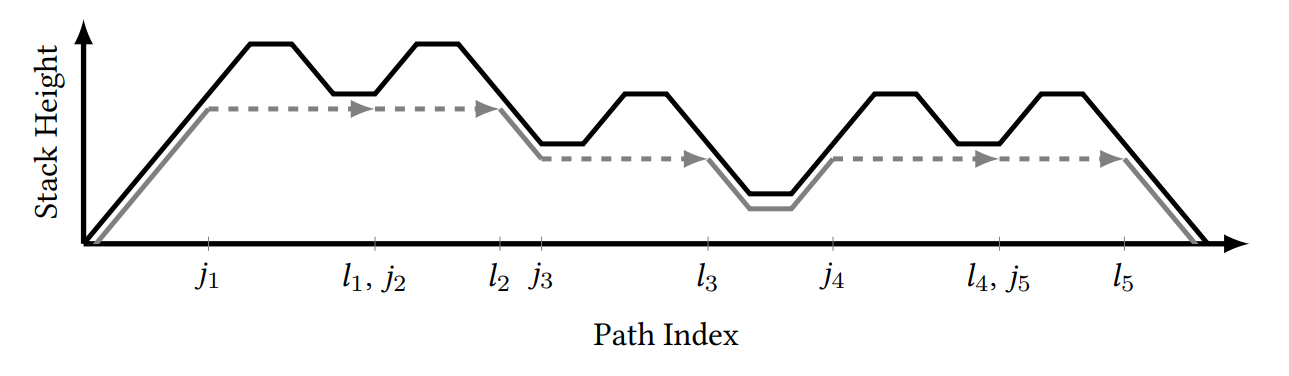
\includegraphics[width=0.75\linewidth]{img/dyck1_path.png}

    Сжимаем bell-shaped пути в $\eps$-рёбра. Снова ищем и снова сжимаем. После каждого сжимания мы убираем все локальные максимумы. Чем больше был максимум, тем длиннее $\eps$-ребро. Хуже всего, когда все новые рёбра длины 2. В любом случае путь становится короче хотя бы в 2 раза, так что таких итераций потребуется не более $\log n^2$ (есть лемма, что найдётся путь длины не более $\O(n^2)$). 

    \item Двунаправленные графы и язык Дика

    Существует несколько частных решений для задачи Диковой достижимости на двунаправленных графах:

    \begin{itemize}
        \item Деревья \cite{Yuan09}

        $\O(n \log n \log k)$~--- центроиды + внутри что-то идейное

        \item Общий случай \cite{Chatterjee17}

        Решение основано на двух фактах. Первый: в двунаправленном графе формируются компоненты Диковой достижимости. Второй: если есть две вершины $u, v$ и компонента Диковой достижимости $C$, такие что $u \xrightarrow{\alpha_i} C$ и $v \xrightarrow{\alpha_i} C$, то $u$ и $v$ тоже лежат в одной компоненте Диковой достижимости. 

        Пользуясь этими фактами, алгоритм с помощью СНМ'а поддерживает компоненты Диковой достижимости и исходящие из них рёбра, чтобы быстро искать новые пары вершин, принадлежащих одной компоненте.

        Итоговая асимптотика алгоритма $\O(m + n \alpha(n))$.
    \end{itemize}

    \item Interleaved Dyck-reachability

        Алгоритм за $\O(n^7)$ для $D_1 \bigodot D_1$ достижимости на bidirected графах~\cite{Li21}

        \textit{Там $\O(n^7)$, потому что авторы~--- дурачки, не умеют рёбра в графе посчитать}

        \textit{Ну или я дурачок, там одно из двух}

        \textit{Было ещё про это (там, вроде, про один из языков сказали, что он bounded, поэтому можно пересекать с регулярным): 
        \url{https://dl.acm.org/doi/pdf/10.1145/3296979.3192378}}
        \TODO: \textit{надо прочитать, что там пишут...}

    \item Граф-цепочка $\O(n^{\omega})$ \cite{Valiant1975}

        CFPQ на графе-цепочке~--- просто задача КС-распознавания (CF-recognition). А она решается за перемножение булевых матриц \cite{Valiant1975}

    \item Ацикличный граф $\O(n^{\omega})$ \cite{Yannakakis1990}

        Ацикличный граф~--- это почти бамбук (= цепочка), нужно только его потопсорить (и где-то ещё быть аккуратным, я не совсем помню сведение)

    \item Bounded-stack RSM $\O(n^3 k^3 / \log^2)$ \cite{Chaudhuri08}

        RSM, который не уходит в рекурсию (т.е. есть из конца ребра $\xrightarrow{S}$ не достижимо никакое ребро $\xrightarrow{S}$)

        Тут применяется какое-то более хитрое (я ещё не разбиралась) итеративное транзитивное замыкание (что-то с dfs'ом, а потом ещё 4 русских сверху, кажется)

    \item Hierarchical FSM $\O(n^{\omega} k^{\omega})$ \cite{Chaudhuri08}

        RSM, в котором боксы упорядочены (топсорт) и бокс с меньшим номером содержит рёбра только с вызовами боксов с большим номером. Задают регулярный язык, но размер FSM может быть экспоненциальным относительно размера RSM.

        Алгоритм идёт в порядке, обратном топсорту, и считает транзитивное замыкание внутри бокса, чтобы провести все рёбра, которые ему соответствуют.

\end{enumerate}

% \subsection{Приложения}

% \textit{Эта часть не для диплома, а для души, потом она в сжатом виде переедет в introduction}

% \begin{itemize}

%     \item Базы данных

%     Querying and storing large volumes of data is an ever-actual concern in computing. Relational databases have been successfully used by the database community and achieved great maturity over the last 40 years [6, 11]. The success of the relational database model relies on a well structured data representation and management, as well as on the use of a (very intuitive and widely used) declarative query language.

%     \item Статический анализ



% \end{itemize}


\subsection{Выводы и результаты по главе}

\TODO
\section{Алгоритм, основанный на пересечении грамматик}

\subsection{Основные определения (пререквизиты)}

\begin{definition}[Конечный автомат (?)]
    НКА и ДКА
    
\end{definition}

\begin{definition}[Рекурсивный конечный автомат (РКА)]
    \textit{Для простоты тут будет немного не такое определение, как в~\cite{Alur05}}

    Это набор компонент $M_1, M_2, \dots , M_k$, где каждая компонента $M_i$~--- это пятёрка $\langle Q_i, \Sigma_i, En_i, Ex_1, \delta_i \rangle$, где 
        \begin{itemize}
            \item $Q_i$~--- конечное множество состояний
            \item $\Sigma_i$~--- конечный алфавит
            \item $En_i \subset Q_i$~--- множество начальных состояний
            \item $Ex_i \subset Q_i$~--- множество конечных состояний
            \item $\delta_i \colon Q_i \times (\Sigma_i \cup \bigcup\limits_{j = 1}^k En_i \times Ex_i ) \to Q_i$~--- функция перехода. У $\delta_i$ есть два типа переходов: \textit{внутренние}, которые работаю как обычные переходы в НКА и \textit{рекурсивные}, которые делают вызов другой компоненты (при этом обозначая начальную и конечную вершину в ней).
        \end{itemize}

    Неформально, это набор компонент, каждая из которых представляет собой ДКА, на рёбрах которого могут быть ``рекурсивные вызовы'' других компонент.

    \TODO: картинка с примером
    
\end{definition}

\begin{definition}[Прямое произведение автоматов]
\end{definition}

\begin{definition}[Транзитивное замыкание]
\end{definition}

\begin{definition}[Инкрементальное транзитивное замыкание]
\end{definition}

\subsection{Описание алгоритма}

\subsubsection{Алгоритм П}

    \textit{Я буду называть его алгоритм П} 

    \TODO: сделать на него ссылки везде

    В данном разделе будет подробно описан алгоритм, предложенный в~\cite{Orachev20}, в модификации которого будет состоять дальнейшая работа.

    Главное идеей алгоритма является следующее замечание: любой помеченный граф можно рассматривать как НКА, в котором не обозначены начальное и конечные состояния. При этом, если зафиксировать конкретные вершины $s$ и $t$ как стартовое и конечное состояние, то полученный автомат будет задавать язык слов $w$, таких что существует путь из $s$ в $t$, на котором читается $w$. 

    \TODO: картинка с примером

    \begin{proposition} \cite{Hopcroft1979}

    Автомат $A$ (НКА/ДКА), построенный как прямое произведение автоматов $A_1$ и $A_2$ ($A = A_1 \otimes A_2$), распознаёт язык, равный пересечению языков $A_1$ и $A_2$ ($\cool{L}(A) = \cool{L}(A_1) \cap \cool{L}(A_2)$)

    \end{proposition}

    Данное утверждение остаётся верным, если один из языков задан РКА~\cite{Beigel}.

    \begin{example}[Построение пересечения РКА и помеченного графа (НКА)]
        РКА для грамматики, задающей язык слов, содержащих равное число букв $a$ и $b$. Может быть задана следующими продукциями:

        $S \to \eps~|~aA~|~bB$

        $A \to bS~|~aAA$
        
        $B \to aS~|~bBB$

        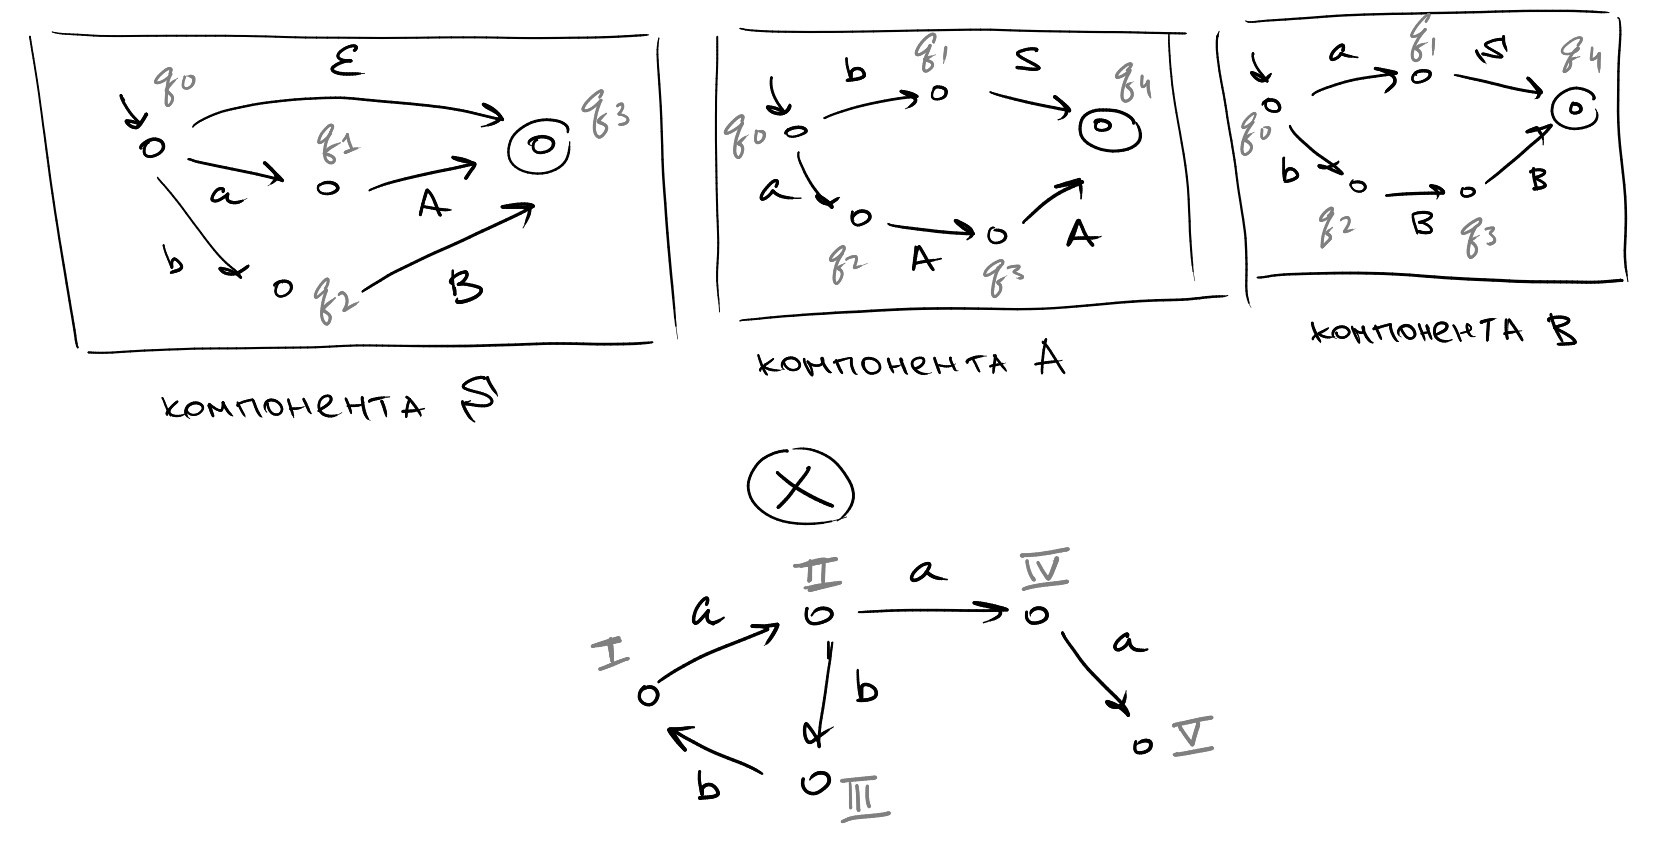
\includegraphics[width=1\linewidth]{img/example_intersection1.png}

        \TODO: дорисовать пример (а потом перерисовать)


    \end{example}

    Так что Алгоритм П можно описать так:
    \begin{enumerate}
        \item Построим прямое произведение входной грамматики $\cool{R}$ и входного графа $G$: $\cool{P} = \cool{R} \otimes G$.
        \item Решим задачу достижимости для полученного РКА $\cool{P}$
        \item Из вершины $u$ в вершину $v$ входного графа существует путь, выводимой входной грамматикой $\cool{G}$ $\EQ$ в $\cool{P}$ есть путь из стартового состояния $(q_0, u)$ в конечное состояние $(q_f, v)$
    \end{enumerate}

    Рассмотрим внимательнее второй пункт~--- задачу достижимости для РКА. В случае обычного автомата эта задача эквивалентна задаче построения транзитивного замыкания~\cite{Yannakakis1990}. В случае же РКА задача осложняется наличием рекурсивных вызовов, которые разрешаются итеративно. (??)

    В листинге~\ref{algo:P} приведён псевдокод Алгоритма П.

    \TODO: что-то написать про епс-переходы

    \begin{algorithm}[H]
        \floatname{algorithm}{Listing}
        \begin{algorithmic}[1]
        \caption{Алгоритм достижимости для РКА}
        \label{algo:P}
        \Function{RSMReachability}{$\cool{R}$}
            \State{$A \gets$ Adjacency matrix for $\cool{R}$}
            \While{$A$ is changing}
                \State{$A' \gets \textit{transitiveClosure}(A)$}
                \For{$i \in 1..k$}
                   \For{$u \in En_i$}
                        \For{$v \in Ex_i$}
                            \If{$A'_{u,v} \wedge \overline{A_{u,v}}$}
                                \State{$A' \gets A' \cup getEdges(i, u, v)$}
                            \EndIf
                        \EndFor
                   \EndFor
                \EndFor
                \State{$A \to A'$}
            \EndWhile
        \State \Return $A$
        \EndFunction
        \end{algorithmic}
    \end{algorithm}

    Работа происходит над матрицей смежности $\cool{R}$~--- изначально туда записываются все ``внутренние'' (нерекурсивные) рёбра. 

    Далее, внешний цикл повторяется, пока матрица смежности $A$ меняется (т.е. пока добавляются новые рёбра). На каждой итерации считается $A'$~--- транзитивное замыкание $A$. После этого находятся все новые пути вида $\langle$стартовое состояние$\rangle$ $\path$ $\langle$конечное состояние$\rangle$~--- те рёбра между стартовой и конечной вершинами компоненты, которых не было в $A$, но которые есть в $A'$~--- и добавляются соответствующие этим путям рёбра: для нового пути $(u \in En_i) \path (v \in Ex_i)$ проводятся все рёбра, соответствующие рекурсивным вызовам $i$-ой компоненты с начальной вершиной $u$ и конечной вершиной $v$.

\subsubsection{Алгоритм П2}

    Можно заметить, что не очень осмысленно на каждой итерации заново считать транзитивное замыкание, достаточно искать только пути, проходящие через рёбра, добавленные непосредственно на предыдущей итерации. То есть достаточно решать задачу {\bf инкрементального} транзитивного замыкания. 

    В листинге~\ref{algo:P2} приведён псевдокод Алгоритма П2 (основанного на инкрементальном ТЗ)

    \begin{algorithm}[H]
        \floatname{algorithm}{Listing}
        \begin{algorithmic}[1]
        \caption{Алгоритм достижимости для РКА (2)}
        \label{algo:P2}
        \Function{RSMReachability2}{$\cool{R}$}
            \State{$A \gets$ Empty adjacency matrix}
            \State{$Q \gets$ Empty Queue}
            \For{$i \in 1..k$}
                \For{$u \xrightarrow{c} v \in \delta_i$}
                    \State{$Q.Push(\langle u, v, i \rangle)$}
                \EndFor
            \EndFor
            \While{$Q$ is not Empty}
                \State{$\langle u, v, i \rangle \gets Q.Pop()$}
                \If{$u \in En_i \wedge v \in En_i$}
                    \Comment{Нашли новый путь}
                    \State{$A \gets A \cup getEdges(i, u, v)$}
                    \State{$Q.PushAll(getEdges(i, u, v))$}
                    \Comment{Добавляем новые рёбра}
                \EndIf
                \For{$x \in Q_i$}
                    \If{$A_{x, u} \wedge \overline{A_{x, v}}$}
                        \For{$y \in Q_i$} 
                            \If{$A_{v, y} \wedge \overline{A_{x, y}}$}
                                \State{$A \gets A \cup \langle x, y \rangle$}
                                \State{$Q.Push(\langle x, y, i \rangle)$}
                                \Comment{Обновлем транзитивное замыкание}
                            \EndIf
                        \EndFor
                    \EndIf
                \EndFor
            \EndWhile
        \State \Return $A$
        \EndFunction
        \end{algorithmic}
    \end{algorithm}

    В алгоритме используется (более менее) стандартная реализация инкрементального транзитивного замыкания~\cite{Ibaraki1983}. Для этого в ходе работы алгоритма поддерживается рабочая очередь $Q$ рёбер транзитивного замыкания, которые были найдены, но ещё не обработаны. 

    При обработке очередного \textit{(потому что оно из очереди ахахах)} ребра, ищутся новые пути, которые проходя через него. А именно, пусть было добавлено ребро $u \to v$. Тогда далее перебирается вершина $x$, такая что из неё была достижима вершина $u$ ($x \path u$), но не была достижима вершина $v$ ($x \not\path v$). Из такой вершины $x$ становятся достижимы все вершины $y$, которые были достижимы из $v$ ($v \path y$).

    Также, как и в Алгоритме П, если ребро ТЗ (= путь в графе) соединяет начальную и конечную вершину, в очередь добавляются также все соответствующие ему рекурсивные рёбра.

    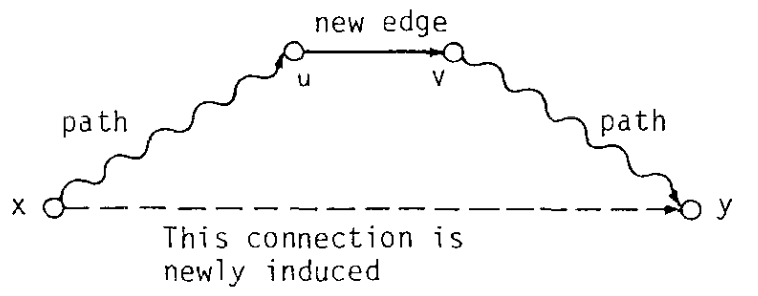
\includegraphics[width=1\linewidth]{img/TC_add.png}

    \TODO: норм картинка

    % Then algorithm iterates while matrix $M_2$ is changing. On each iteration the Kronecker product $M_3$ of matrices $M_1$ and $M_2$ is computed (that is adjacency matrix of Kronecker product $R \otimes \mathcal{G}$). After that, transitive closure $C_3$ of the product $M_3$ is computed. Then algorithm iterates over newly added edges (after transitive closure) and if one $(q_s, u) \rightsquigarrow (q_f, v)$ connects initial and final states of the same RSM box $S$, then new edge $u \xrightarrow{S} v$ is added. 
    
\subsection{Время работы}

\subsubsection{Алгоритм П}

\subsubsection{Алгоритм П2}

\subsection{Выводы и результаты по главе}

\section{Результаты (1)}\label{section:bidirected}

В данном главе будет рассмотрена модификация алгоритма~\ref{algo:PI}, основанная на ослаблении условия на граф, а именно, на ``предположении'', что он является неориентированным. Также будет доказана корректность данной модификации для двунаправленных графов и языка Дика, а также для неориентированных графов и некоторых видов грамматик.

Для неориентированных графов отношение достижимости равно отношению ``принадлежать одной компоненте связности''. Поддерживать добавление рёбер и проверку связности в неориентированном графе можно с помощью структуры данных Система Непересекающихся Множеств. 

% Система Непересекающихся Множеств (СНМ)
\begin{definition}
  \textit{Система Непересекающихся Множеств (или СНМ)}\footnote{Disjoint-set/union–find data data structure}~\cite{Galler1964}~--- структура данных для работы с непересекающимися множествами. Её интерфейс включает следующие операции:
  \vspace{-\topsep}
  \begin{itemize}
    \setlength\itemsep{-0.1em}
    \item \textit{MakeSet}$(x)$~--- создаёт новое множество, состоящее из одного элемента $x$
    \item \textit{Find}$(x)$~--- возвращает элемент-представитель множества, содержащего $x$. Для всех элементов одного множества элемент-представитель одинаков
    \item \textit{Union}$(x, y)$~--- объединяет множества, содержащие элементы $x$ и $y$
  \end{itemize}
\end{definition}

\subsection{Алгоритм, основанный на неориентированном транзитивном замыкании}

В листинге~\ref{algo:NP} приведён псевдокод алгоритма.

\begin{algorithm}[H]
  \floatname{algorithm}{Listing}
  \begin{algorithmic}[1]
  \caption{Алгоритм достижимости для РКА, основанный на неориентированном ИТЗ}
  \label{algo:NP}
  \Function{UndirectedRSMReachability}{$\cool{R}$}
      \State{$A \gets$ Empty adjacency matrix}
      \State{$Q \gets$ Empty Queue}
      \State{$D \gets$ DSU($|\bigcup\limits_{i=1}^k Q_i|$)}
      \For{$i \in 1..k$}
          \For{$u \xrightarrow{c} v \in \delta_i$}
              \State{$Q.Push(\q{u, v, i})$}
          \EndFor
      \EndFor
      \While{$Q$ is not Empty}
          \State{$\q{u, v, i} \gets Q.Pop()$}
          \If{$u \in En_i \wedge v \in En_i$}
              \Comment{Нашли новый путь}
              \State{$A \gets A \cup getEdges(i, u, v)$}
              \State{$Q.PushAll(getEdges(i, u, v))$}
              \State{$D.Union(u, v)$}
              \Comment{Добавляем новые рёбра}
          \EndIf
      \EndWhile
  \State \Return $A$
  \EndFunction
  \end{algorithmic}
\end{algorithm}

Для реализации используются две вспомогательные структуры данных: очередь $Q$, хранящая рёбра, которые были добавлены в граф, но ещё не обработаны (как и в оригинальном алгоритме), и СНМ $D$, поддерживающая компоненты связности и поиск новых путей $\langle$стартовое состояние$\to$конечное состояние$\rangle$. 

Опишем подробно структуру используемой СНМ (в листинге~\ref{algo:DSU} приведён псевдокод).

\algblockdefx[Structure]{Structure}{EndStructure}
[1]{{\bf Structure} #1}
{}

\begin{algorithm}[H]
  \floatname{algorithm}{Listing}
  \begin{algorithmic}[1]
  \caption{Система Непересекающихся Множеств}
  \label{algo:DSU}
  \Structure{DisjointSets}
      \Function{DisjointSets}{$V$}
          \For{$v \in V$}
              \State{$P[v] \gets v$}
              \Comment{Предкок}
              \State{$R[v] \gets 0$}
              \Comment{Ранг}
          \EndFor
          \For{$v \in En(V)$}
              \State{$En[v] \gets \{v \}$}
              \Comment{Список стартовых вершин поддерева}
          \EndFor
          \For{$v \in Ex(V)$}
              \State{$Ex[v] \gets \{v \}$}
              \Comment{Список конечных вершин поддерева}
          \EndFor
      \EndFunction
      \Function{Find}{$v$}
          \If{$P[v] = v$}
              \Return $v$
          \EndIf
          \Return $P[v] = Find(P[v])$
          \Comment{Эвристика сжатие путей}
      \EndFunction
      \Function{Union}{$u, v$}
          \State{$u \gets Find(u)$}
          \State{$v \gets Find(v)$}
          \If{$u = v$}
              \Return
          \EndIf
          \If{$R[u] > R[v]$}
              \State{$Swap(u, v)$}
              \Comment{Ранговая эвристика}
          \EndIf
          \State{$Q.PushAll(\{ \q{en_u, ex_v}~|~en_u \in En[u], ex_v \in Ex[v] \})$}
          \State{$Q.PushAll(\{ \q{en_v, ex_u}~|~en_v \in En[v], ex_u \in Ex[u] \})$}
          \Comment{Добавление новых рёбер}
          \State{$En[v] \gets En[v] \cup En[u]$}
          \State{$Ex[v] \gets Ex[v] \cup Ex[u]$}
          \State{$R[v] \gets \max(R[v], R[u]+1)$}
          \State{$P[u] = v$}
          \Comment{Объединение компонент}
      \EndFunction
  \EndStructure
  \end{algorithmic}
\end{algorithm}

За основу взята стандартная реализация \cite{Hopcroft1973} на подвешенных деревьях, использующая обе эвристики: сжатие путей и ранговую. 

% \TODO: \textit{Надо ли её расписывать?}
% Ненадо

Дополнительно в корнях хранятся списки всех начальных и конечных состояний компоненты. При добавлении ребра в операции \textit{Union} перебираются все пары начальная/конечная вершина из двух компонент и соответствующие им рёбра добавляются в рабочую очередь $Q$. 

\TODO: (подумоть) можно ли добавлять сразу много рёбер и сжимать их дфсом (как Борувка)?

\subsection*{Время работы}

\begin{theorem}
  На РКА из $|V|$ состояний и $|E^{*}|$ рёбрах в транзитивном замыкании, алгоритм~\ref{algo:NP} отработает за время $\O(|V| + |E^{*}| \alpha(|V|))$
\end{theorem}

\begin{proof}
  Как и в алгоритме~\ref{algo:PI} проход по внешнему циклу и добавление новых рекурсивных рёбер отработает за $\O(|E^{*}|)$, так как каждое ребро транзитивного замыкания рассмотрится не более одного раза.

  Осталось оценить время работы $|E^{*}|$ вызовов функции \textit{Union}. Каждый из них совершает 2 вызова функции \textit{Find}, каждый из которых отработает за амортизированное $\alpha(|V|)$. Также, если вершины находились в разных компонентах, происходит перебор всех пар начальное-конечное состояние. Однако, этот перебор суммарно переберёт каждое ребро транзитивного замыкания не более одного раза, так что суммарно отработает за $\O(|E^{*}|)$.

  Итого, время работы алгоритма составляет $\O(|V| + |E^{*}| \alpha(|V|))$ ($\O(|V|)$ берётся из создания СНМ на $|V|$ множеств). 
\end{proof}

\subsection{Корректность для неориентированных графов и некоторых классов грамматик}

\TODO: может, в мусорку этот subsection?

\subsection{Корректность для двунаправленных графов и языка Дика}

\textit{Напоминание, что для языка Дика контекстно-свободная достижимость $\to$ Дикова достижимость}

Для доказательства потребуется следующее вспомогательное утверждение

\begin{lemma}\label{lemma:bidir_equiv}
  Для вершин двунаправленных графов отношении Диковой достижимости является отношением эквивалентности.
  % For bidirected graphs the Dyck-reachability relation forms an equivalence, i.e., for all bidirected graphs $G$, for every pair of nodes $u$, $v$, we have that $v$ is Dyck-reachable from $u$ iff $u$ is Dyck-reachable from $v$.
\end{lemma}
\begin{proof}
  ~\\
  \TODO: ну тут тупо

\end{proof}

\begin{note}    
  Для данного алгоритма будем использовать следующий вид грамматики для языка Дика:

  $S \to \eps~|~SS~|~(_1 S )_1~|~ \dots ~|~(_k S )_k$

  \begin{figure}[H]
      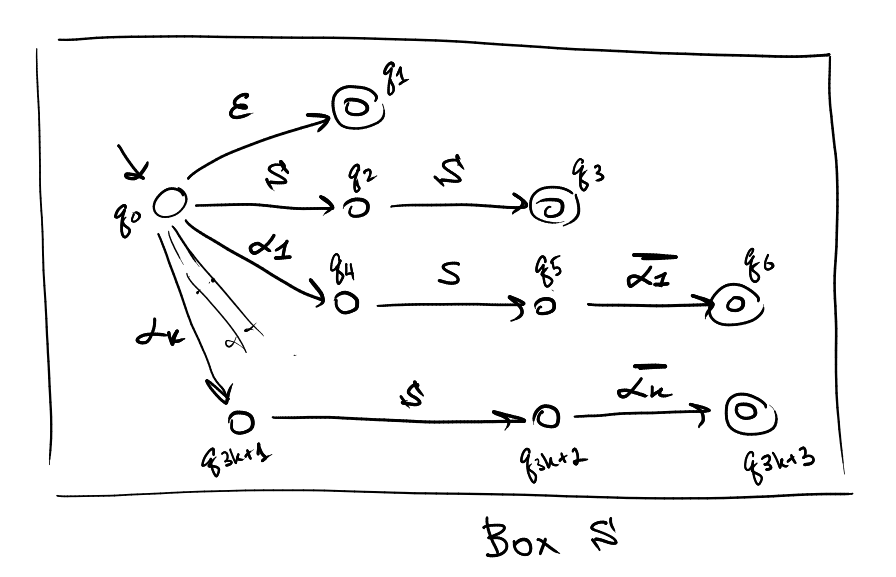
\includegraphics[width=0.75\linewidth]{img/dyck_box}
      \caption{РКА для языка Дика}
      \label{img:dyck_rsm}
  \end{figure}

  На рисунке~\ref{img:dyck_rsm} приведена РКА для данной грамматики. Заметим, что он содержит всего одну компоненту ($S$).

  \TODO: нарисовать красиво

\end{note}


\begin{theorem}
  Решение для CFPQ, использующее Алгоритм НП, работает корректно на двунаправленных графах и языке Дика.
\end{theorem}

\begin{proof}

  Достаточно доказать, что для любой пары состояний $u \in En_i, v \in Ex_i$ существование неориентированного пути эквивалентно существованию ориентированного.

  % We only need to prove, that for every pair $u, v \in V(\mathcal{G})$ there is a path $(q_s, u) \rightsquigarrow (q_{f_i}, v)$ in ({\bf directed}) Kronecker product $G \otimes \mathcal{G}$ 
  % iff 
  % there is such path $(q_s, u) \rightsquigarrow (q_{f_j}, v)$ in an {\bf undirected} product (there $q_s$ is the initial state and $q_{f_i}, q_{f_j}$ are some final states of $G$ respectively).

  $\Leftarrow$ (ориентированный $\SO$ неориентированный)

  Очевидно, если есть ориентированный путь $u \path v$, то ровно если убрать ориентацию этот путь никуда не денется.

  % Obviously (if $(q_{f}, v)$ is reachable from $(q_{s}, u)$ by directed edges, it is all the more reachable by undirected edges).

  $\Rightarrow$ (неориентированный $\SO$ ориентированный)

  % Для начала

  At first, note that the Kronecker product $G \otimes \mathcal{G}$ forms some kind of a layered structure~--- $i$-th layer consists of vertices $(q_i, v)$, where $q_i$ is $i$-th RSM state. Because RSM is topologically sorted ({\color{red}{TODO}}), every edge $(q_i, u) \rightarrow (q_j, v)$ goes forward.

  We will call path \textit{simple} if it visits every layer no more than once.

  We prove the claim by induction on the $l$ (path length).

  Clearly the result is true for $l \le 3$, because the only way to achive final vertex in $1, 2$ or $3$ edges is by a simple vertical path (which exists in the original graph too).

  Otherwise (if $l \ge 4$), path is not simple. 

  Consider the first flex point of the path, that is the vertex $(q_i, v)$ such that edges $(q_j, u) \rightarrow (q_i, v)$ and $(q_i, v) \rightarrow (q_k, w)$ are in the path and $j, k \le i$ (so, the path is convex at this point).

  Looking at the grammar graph we can notice, that every state has indegree $\le 1$. So at the flex point there are actually two same-labeled edges (that is, $j = k$). 

  There can be three different types of labels on those edges:

  \begin{itemize}
    \item $\alpha_l$-label

      \textit{path: $(q_0, u) \rightarrow (q_i, v) \rightarrow (q_0, w) \rightarrow \dots \rightarrow (q_f, z)$.}

      Since $\alpha_l$-labeled edges could only be added on the initialization stage, 
      graph $\mathcal{G}$ contains edges $u \xrightarrow{\alpha_l} v$ and $w \xrightarrow{\alpha_l} v$. Notice, that cause $\mathcal{G}$ is bidirected, it also has to contain edges $v \xrightarrow{\overline{\alpha_l}} u$ and $v \xrightarrow{\overline{\alpha_l}} w$.

      Now we can notice, that $w$ is Dyck-reachable (by the path $\alpha_l \overline{\alpha_l}$) from $u$, so there is an $S$-labeled edge from $u$ to $w$. We can also conclude, that (by induction) there is a directed path from $(q_0, w)$ to $(q_f, z)$ (there $z$ is the end of the path and $q_f$ is some final state of $G$), so there is an $S$-labeled edge from $w$ to $z$. 

      Using this two observation we can construct a directed path from $u$ to $z$: $u \xrightarrow{S} w \xrightarrow{S} z$. 
    \item $S$-label

      \textit{path: $(q_0, a) \rightarrow \dots \rightarrow (q_j, u) \rightarrow (q_i, v) \rightarrow (q_j, w) \rightarrow \dots \rightarrow (q_f, z)$.}

      $\mathcal{G}$ contains $S$-labeled edges $u \xrightarrow{S} v$ and $w \xrightarrow{S} v$. Since $\mathcal{G}$ is bidirected, then by \ref{r1} $v \xrightarrow{S} u$ and $v \xrightarrow{S} w$. Combining $u \xrightarrow{S} v$ and $v \xrightarrow{S} w$ we get that $u \xrightarrow{S} w$. 

      No we want to sort of contract this edge, joining $u$ and $w$ (on the $j$-th level). Then we can get (by induction hypothesis) the directed path from $(q_0, a) \rightsquigarrow (q_f, z)$. If new path does not contain joined $uw$ vertex, then that's the answer. Otherwise we can split this vertex back, inserting between $u$ and $w$ the $S$-labeled path (that one, from $u \xrightarrow{S} w$ edge). We can do it, because the both of these paths form correctly matched parenthesis ({\color{red}{TODO}}: we can prove this using stack-based checking algorithm).

      \textit{Two other cases can be proved the same way, but I find it a little dishonest}

    \item $\overline{\alpha_l}$-label

      \textit{path: $(q_0, a) \rightarrow \dots \rightarrow (q_j, u) \rightarrow (q_f, v) \rightarrow (q_j, w) \rightarrow \dots \rightarrow (q_f, z)$.}

      Since $\alpha_l$-labeled edges could only be added on the initialization stage, 
      graph $\mathcal{G}$ contains edges $u \xrightarrow{\overline{\alpha_l}} v$ and $w \xrightarrow{\overline{\alpha_l}} v$. Notice, that cause $\mathcal{G}$ is bidirected, it also has to contain edges $v \xrightarrow{\alpha_l} u$ and $v \xrightarrow{\alpha_l} w$.

      By induction, we get that $a \xrightarrow{S} v$. Now we will construct a second part of the path: $(q_0, v) \xrightarrow{\alpha_l} (q_{j-1}, w) \xrightarrow{S} (q_j, w) \rightsquigarrow (q_f, z)$ ($q_{j-1}, w) \xrightarrow{S} (q_j, w)$ ~--- initial $S$-loop). By induction, we have directed simple version of this path, so $v \xrightarrow{S} z$. 

      Combining this two paths ($a \xrightarrow{S} v$ and $v \xrightarrow{S} z$) we get $a \xrightarrow{SS} z \Rightarrow a \xrightarrow{S} z$~--- desired path.
        
    \begin{figure}[H]
        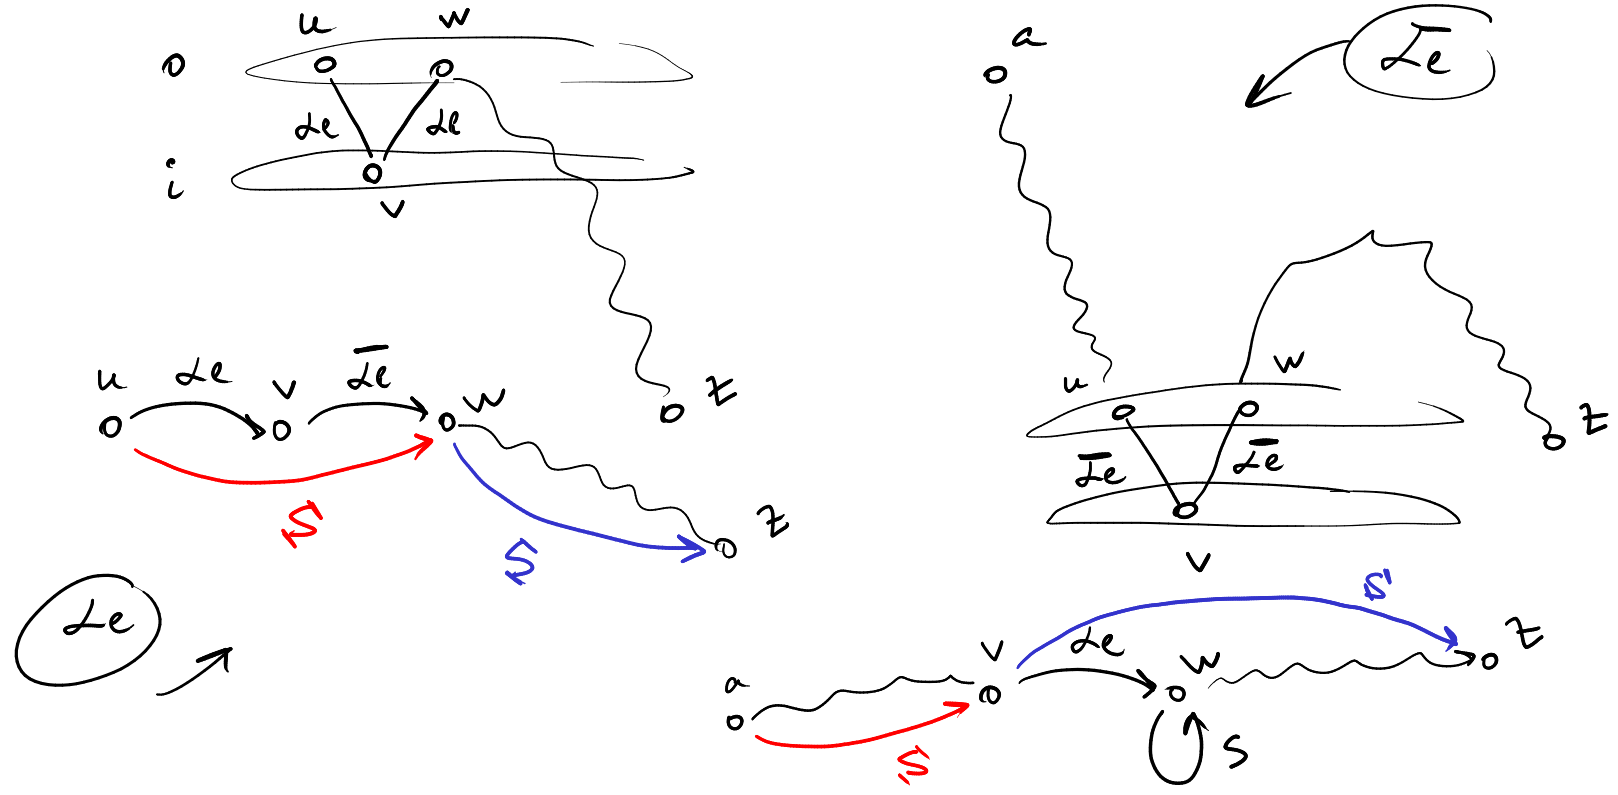
\includegraphics[width=\linewidth]{img/th_proof_img}
    \end{figure}
  \end{itemize}

\end{proof}

\subsection{Выводы и результаты по главе}

\TODO
\section{Результаты (2)}

\subsection{Алгоритм для языка Дика на одном типе скобок}

\begin{note}
  Строки, принадлежащие языку Дика $\cool{D}_1$ часто изображают в виде так называемых \textit{путей Дика}~--- путей из точки $(0, 0)$ в точку $(0, 2n)$, не опускающихся ниже оси абсцисс. Открывающей скобке соответствует вектор $(1, 1)$, закрывающей~--- $(1, -1)$.

  \TODO: Картинка 
\end{note}

\TODO: для semi-dyck тоже работает, нужно это упомянуть

Для построения алгоритма воспользуемся следующим результатом:

\begin{lemma}[Дюлеаж и Лоран~\cite{Deleage1986}]

Для языка $L$ определим $p_L(n)$\footnote{Формально, $p_L(n) = \max \{ \min \{|w| \colon w \in L \cap K \}, K \in Rat_n(X), L \cap K \ne \varnothing \}$,\\ где $Rat_n(X)$~--- регулярные языки над алфавитом $X$, распознаваемые НКА с $\le n$ состояниями.}~--- максимальная длина кратчайшего слова в $L \cap K$ по всем регулярным языкам $K$, задаваемым НКА с $\le n$ состояниями.

Тогда для языка Дика $D_1$ на одном типе скобок $p_{D_1}(n) = \O(n^2)$\footnote{Точная оценка~--- $2n^2 + 4n$}
\end{lemma}

\begin{corollary}
    Для любой пары вершин $u, v \in V(G)$, если есть Диков путь $u \path v$, то существует и Диков путь $u \path v$, длина которого $\O(n^2)$.
\end{corollary}
\begin{proof}
    Слова, читаемые на путях $u \path v$ задаются НКА на $n$ вершинах~--- графом $G$, в котором $u$ и $v$ выбраны за начальное и конечное состояния соответственно.
\end{proof}

\begin{note}
Пользуясь этим фактом, можно соорудить наивный алгоритм~--- достаточно лишь заметить, что раз длина искомого пути всегда ограничена, то можно задать такие пути с помощью ДКА: язык $D_1$ задаётся автоматом с одним счётчиком, значение счётчика не превышает $\O(n^2)$, так что его можно закодировать в состояние. Однако и размер такого ДКА будет $\O(n^2)$, что для данной задач слишком много.
\end{note} 

\TODO: дописать красиво

\textit{Ну тут мотивация простая, если строить автомат по грамматике, то часто он получается экспоненциального размера. Сейчас хотим то же в обратную сторону провернуть. Ещё мотивация: чтобы хранить одну чиселку порядка $n^2$ в считающем автомате нужно всего $\O(\log n)$ бит, так что хочется в такое ограничение и уложиться}\\
\TODO: написать красивые слова

\textit{Хочется тут красивую подводку, но не выходит...}

Хотим использовать Алгоритм П (потому что иначе субкубическое решение не получим), так что нужно, чтобы у нас было мало итераций. С обычной грамматикой ($S \to \eps~|~(S)~|~SS$) ничего хорошего не выйдет: рассмотрим путь $(^k )^k$, чтобы его найти потребуется $k$ итераций. Так что наша цель~--- за малое число итераций (добавления рёбер) находить такие длинные пути.

Строим РКА, компоненты описываются в виде продукций, обсуждалось (\TODO: пока что ещё нет), как строить одно из другого.

Строим $2K$ (где $K = \lceil \log (2 n^2 + 4n) \rceil$) компонент РКА, отвечающих за сжатие вертикальных путей: $U_i$ сжимают пути вида $(^{2^i}$, $D_i$ сжимают пути вида $)^{2^i}$:

$U_0 \to ($

$U_1 \to U_0 S U_0$

$U_2 \to U_1 S U_1$

\dots

$U_K \to U_{K-1} S U_{K-1}$ 

В продукции для $U_i$ есть $S$ между $U_{i-1}$ и $U_{i-1}$~--- она нужна, так как мы ищем не строго возрастающие пути, а допускаем им некоторое время ``идти прямо'' (получаются уже такие пути Моцкина, а не Дика, в которых $S$ соответствуют горизонтальным рёбрам)

Продукции для $D_i$ выглядят аналогично.

Теперь можем строить компоненту, отвечающую за, собственно, пути Дика. Продукция $S \to ( S )$ в обычной грамматике как бы ``сжимала уголки''. Теперь, пользуясь $U_i$ и $D_i$ можем ``сжимать уголки'' побольше.

$S \to \eps~|~U_0 S D_0~|~U_1 S D_1~|~ \dots ~|~U_K S D_K~|~S^*$

Продукция $S \to S^*$ обозначает петлю на терминальной вершине в компоненте $S$ в РКА грамматики (это так называемая, продукция транзитивного замыкания, её предназначение~--- да одну итерацию сжимать все пути из $S$-ок; в произведении с графов она образует клику на терминальных состояних в компоненте).

При оценке асимптотики алгоритма будет важно, что все компоненты РКА имеют константный размер (число состояний), так что разобьём компоненту $S$ на $K$ штук: $S_i \to U_i S D_i$, $S \to (S_0~|~S_1~|~ \dots ~|~ S_k)^*$ (одно стартовое/терминальное состояние, на котором весит $K$ петель).

Собственно, алгоритм~--- запустить алгоритм П (\TODO: линк) на прямом произведении входного графа и описанной выше грамматики.
 % для языка Дика с ограниченной глубиной стека.

% \TODO: \textit{Можно забабахать пример (потому что он получается огромный..) и отправить его в Приложения}

\TODO: \textit{можно сюда просто вставить маленький пример, где рассматривается один путь и показано, как он сжимается, без пересечения с грамматикой.}

% Опишем КС-грамматику, задающую язык Дика на одном типе скобок, вложенность 

\subsection{Пример}

\begin{figure}[H]
    \begin{minipage}[h]{0.47\linewidth}
        \center{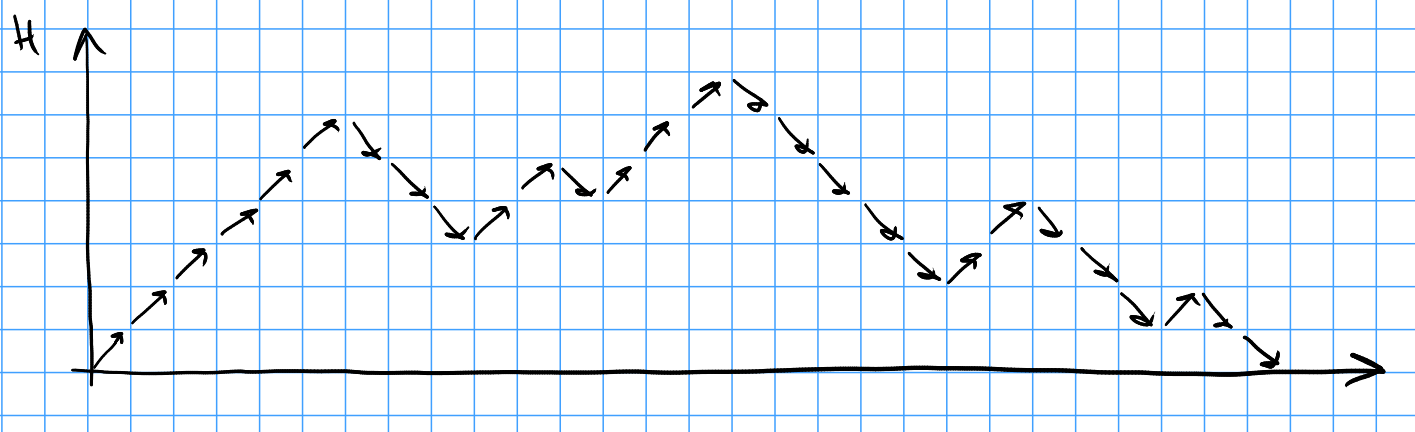
\includegraphics[width=1\linewidth]{img/dyck1_example/phase0}} 0 итерация
    \end{minipage}
    \hfill
    \begin{minipage}[h]{0.47\linewidth}
        \center{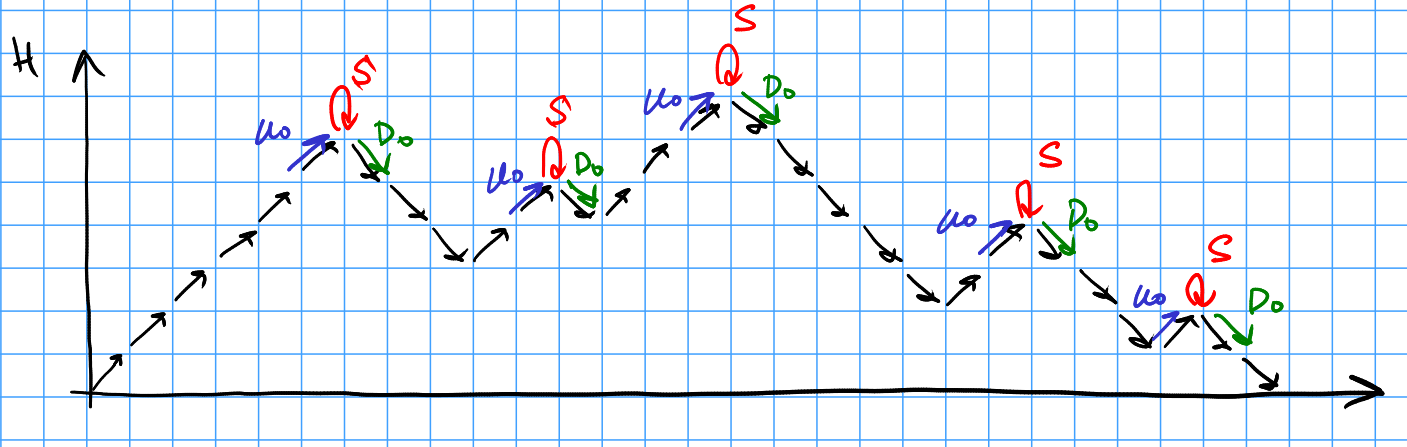
\includegraphics[width=1\linewidth]{img/dyck1_example/phase1}} 1 итерация
    \end{minipage}
    \vfill
    \begin{minipage}[h]{0.47\linewidth}
        \center{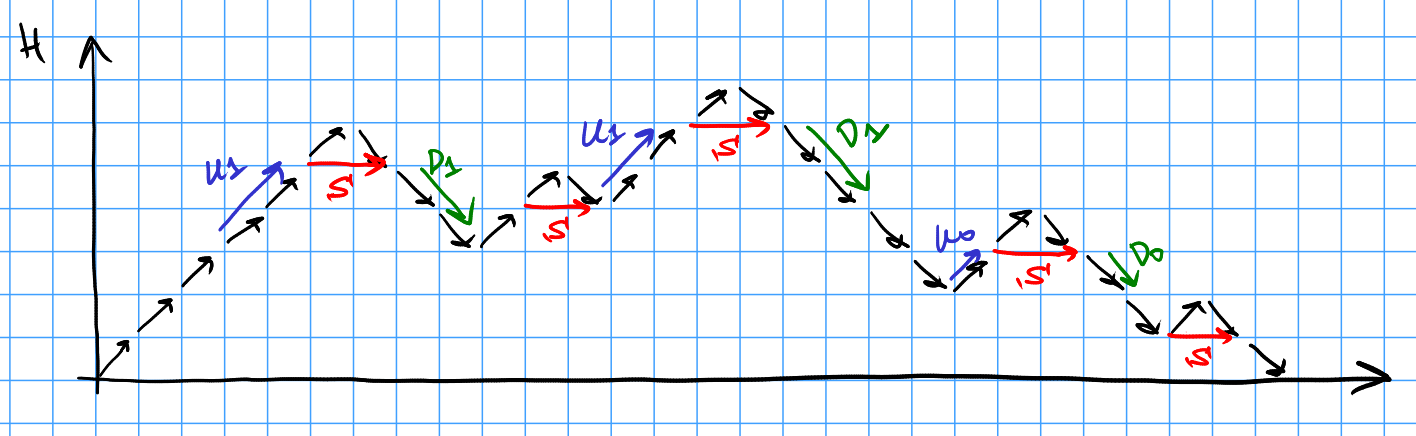
\includegraphics[width=1\linewidth]{img/dyck1_example/phase2}} 2 итерация
    \end{minipage}
    \hfill
    \begin{minipage}[h]{0.47\linewidth}
        \center{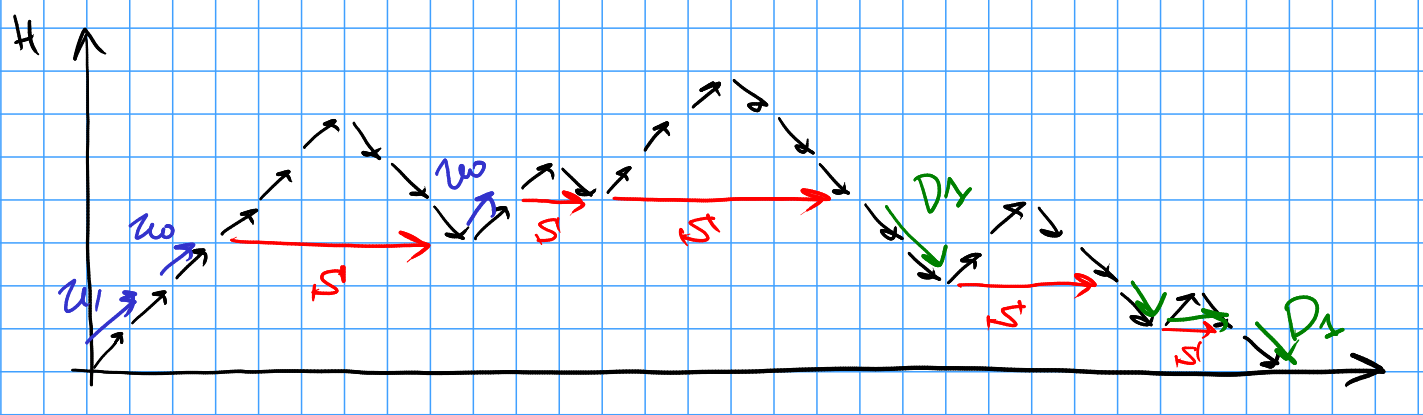
\includegraphics[width=1\linewidth]{img/dyck1_example/phase3}} 3 итерация
    \end{minipage}
    \vfill
    \begin{minipage}[h]{0.47\linewidth}
        \center{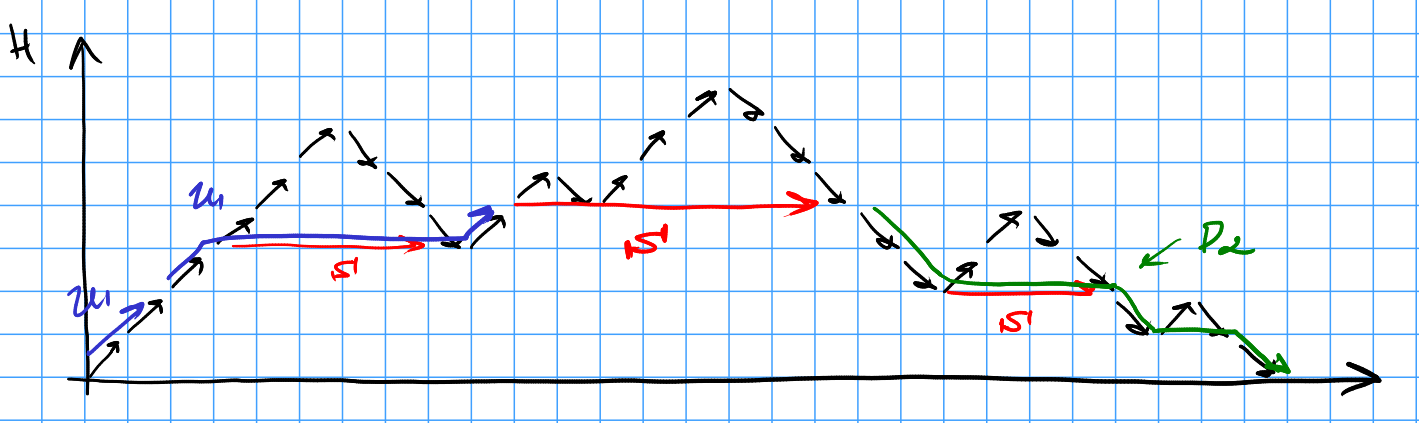
\includegraphics[width=1\linewidth]{img/dyck1_example/phase4}} 4 итерация
    \end{minipage}
    \hfill
    \begin{minipage}[h]{0.47\linewidth}
        \center{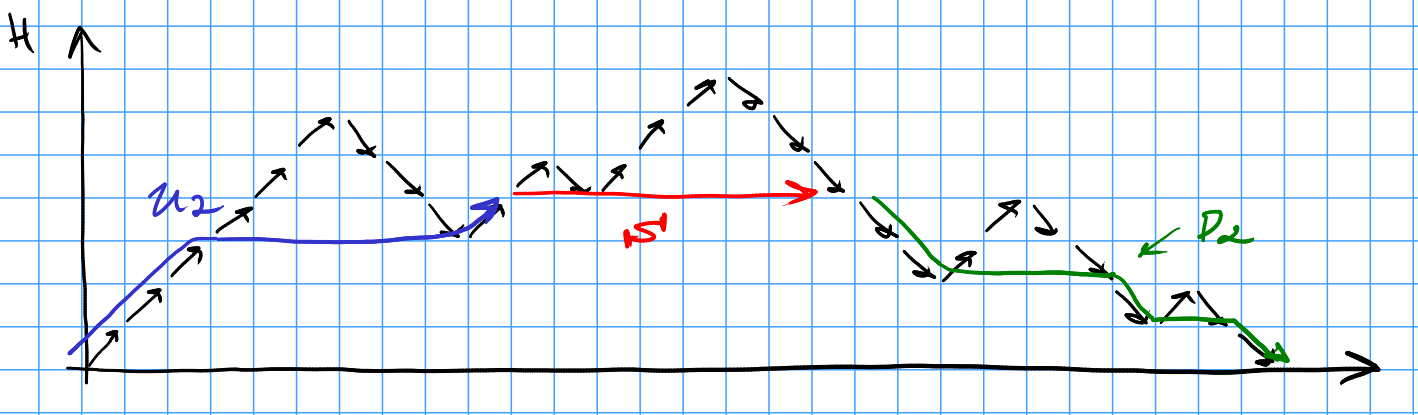
\includegraphics[width=1\linewidth]{img/dyck1_example/phase5}} 5 итерация
    \end{minipage}

    \caption{Пример работы алгоритма (на конкретном пути)}
    \label{img:dyck1_example}
\end{figure}

\subsection{Корректность алгоритма}

\TODO

\subsection{Время работы}

\TODO: \textit{Я сейчас докажу $\O(n^{\omega} \log^3 n)$, но, кажется, можно сократить на лог (засчёт того, что у нас параллельно сжимаются и $S$-ки, и $U$-шки с $D$-шками)}

Для доказательства времени работы нам потребуется пара вспомогательных утверждений.

\begin{lemma}
    После $i$-ой итерации алгоритма 
\end{lemma}

\begin{theorem}
Время работы Алгоритма (link (?)) на языке Дика на одном типе скобок~--- $\O(n^{\omega} \log^3 n)$, где $n$~--- число вершин входного графа.
\end{theorem}

\begin{proof}
Время работы алгоритма П состоит из двух множителей: времени работы одной итерации и числа итераций.

Время работы одной итерации в алгоритме П составляло $\O(N^{\omega})$ (где $N$~--- число состояний РКА-произведения), т.к. на каждой итерации считалось транзитивное замыкание. Заметим, что на самом деле достаточно находить транзитивное замыкание отдельно в каждой компоненте РКА (т.к. разные компоненты вообще не связны). Т.к. компоненты РКА грамматики константны, то размер компонент РКА-произведения~--- $\O(n)$. Так что суммарное время работы одной итерации составит $\O(n^{\omega} K)$.   
% (\TODO: link)~---\\ $O(\langle \text{время работы одной итерации} \rangle \cdot \langle \text{\# итераций} \rangle)$.

Оценим теперь число итераций. 

\TODO: \textit{за лог итераций срезаются все уголки (локальные максимумы), нужно теперь их аккуратно посчитать, смотря на соседей (и минимумы)}

\end{proof}

\begin{note}
Этот результат не обобщается на языки Дика с большим типом скобок. 

Мотивация примерно такая: во1, они сложнее (язык Дика на $\ge 2$ типах скобок~--- такой же мощный как и произвольный КС-язык (теорема Хомского-Шутценбергера, тогда как язык Дика на одном типе скобок вроде как попроще. \textit{Ещё Дик на $\ge 2$ типах скобок генерирует full AFL (Abstract Families of Languages) (что бы это не значило)}), во2, сейчас мы играли на том, что состояние~--- примерно одна чиселка (ну опять-таки, язык Дика на одном типе скобок распознаётся автоматом с одним счётчиком), а для большего типа скобок нужен весь стек.
\end{note}

\subsection{Выводы и результаты по главе}
\section{Результаты (3)}\label{section:dyck_1_1}

\subsection{Алгоритм для смешанного языка Дика}

Смешанный язык Дика $\cool{D}_i \odot \cool{D}_j$ является пересечением двух КС языков, а именно, 
$\cool{D}_i \odot \cool{D}_j = L_1 \cap L_2$, где 
$L_1 : S_1 \to S_1 S_1~|~(_1 S_1 )_1~|~ \dots (_i S_1 )_i ~|~ \eps ~|~ [_1 ~|~ ]_1 ~|~ \dots ~|~ [_j ~|~ ]_j$ и 
$L_2 : S_2 \to S_2 S_2~|~[_1 S_2 ]_1~|~ \dots [_j S_2 ]_j ~|~ \eps ~|~ (_1 ~|~ )_1 ~|~ \dots ~|~ (_i ~|~ )_i$ 
(то есть двух языков Дика, которые игнорируют скобки второго типа). 

Однако КС-языки не замкнуты относительно пересечения: при нём получается конъюнктивный язык~\cite{Okhotin01}, задача достижимости для которого является алгоритмически неразрешимой~\cite{Hellings14}. Более того, она неразрешима уже для языка $\cool{D}_2 \odot \cool{D}_2$ даже на двунаправленных графах~\cite{Li21}. 

Однако задача достижимости для языка $\cool{D}_1 \odot \cool{D}_1$ на двунаправленных графах вполне разрешима, причём за полиномиально время.

В этой главе будет приведён улучшение алгоритма Ли и др.~\cite{Li21} решения этой задачи, основанное на идее пересечения языков.

\begin{note}\label{fact:intersection}

  Здесь и далее будем считать, что первый язык Дика~--- язык круглых ПСП ($\cool{D}_p : S \to SS~|~(S)~|~\eps$), второй~--- язык квадратных ПСП ($\cool{D}_b : T \to T~|~[T]~|~\eps$).
\end{note}

Заметим, что слово принадлежит $\cool{D}_p \odot \cool{D}_b$, тогда и только тогда, когда на любом его префиксе баланс обоих типов скобок неотрицателен, а конечный баланс равен нулю. Баланс строки будем записывать как $(p, b)$, где $p$~--- баланс круглых скобок, а $b$~--- квадратных.

Для решения понадобится следующий вспомогательный факт:

\begin{lemma}{Ли и др.~\cite{Li21}}\label{lm:dyck_6v}
  В двунаправленном графе, если между парой вершин $(u, v)$ существует какой-то $\cool{D}_1 \odot \cool{D}_1$ путь, то существует и такой путь, на котором в любой момент времени вложенность хотя бы одного типа скобок не превышает $6 |V|$.
\end{lemma}

\begin{figure}[h]
  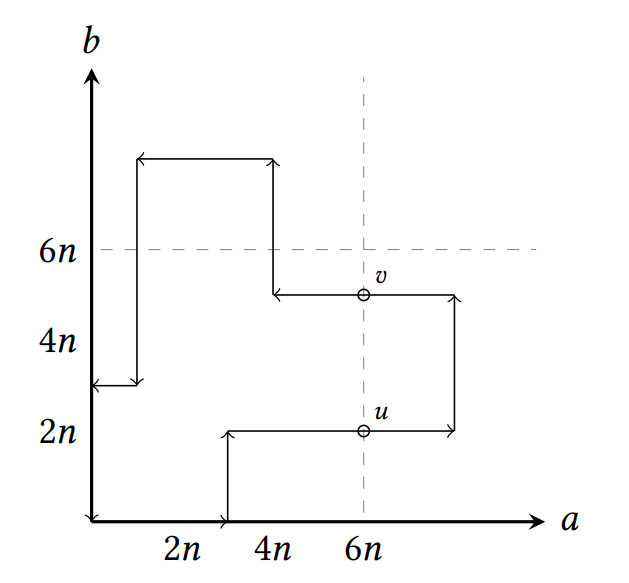
\includegraphics[width=0.75\linewidth]{img/6n_6n_path}
  \caption{Путь в координатах баланса}
  \label{img:6v_path}
\end{figure}

\TODO: картиночька

Нарисуем~(рис.~\ref{img:6v_path}) такой (как в утверждении леммы~\ref{lm:dyck_6v}) путь на плоскости, где первая координата~--- баланс круглых скобок, вторая~--- баланс квадратных (т.е. просто $p$ и $b$). Тогда во-первых, весь путь будет проходить в первой четверти. Во-вторых, он не будет заходить (найдётся такой, что не будет заходить, и мы ищем именно его) в сектор $[6|V|+1, +\oo) \times [6|V|+1, +\oo)$
    
То есть путь можно искать следующего вида: он в основном проходит внутри квадрата $[0, 6|V|] \times [0, 6|V|]$, иногда выходя из него, но только по одной координате (т.е. либо в сектор $[0, 6|V|] \times [6|V| + 1, +\oo)$, либо в сектор $[6|V| + 1, +\oo) \times [0, 6|V|]$).

Тогда можно искать отдельно две эти сущности: куски путей внутри квадрата $[0, 6|V|] \times [0, 6|V|]$, и куски путей снаружи.

% Т.е. нужно разобрать отдельно две сущности: куски путей внутри квадрата, и куски путей, которые выходят погулять.

Вооружившись этим знанием, построим алгоритм:

\begin{enumerate}
    \item {\bf Часть пути, лежащая в квадрате $\mathbf{[0, 6|V|] \times [0, 6|V|]}$}

    Внутри квадрата ограничена вложенность обоих типов скобок. Помним из прошлой главы (замечание~\ref{fact:regular_cfpq}), что в случае ограниченной вложенности язык получается регулярным. Строим автоматы для таких регулярных языков: $\cool{D}_p^{6|V|}$ и $\cool{D}_b^{6|V|}$, оба размера $\O(n)$.

    Пересекая оба этих языка и входной граф получаем автомат, состояние в котором~--- тройка $\q{v, p, b}$ (вершина и два баланса). Размер автомата: $\O(|V|^3)$ вершин, $\O(|E||V|^2)$ рёбер.

    Также в этом автомате нужно провести $\eps$-рёбра, соответствующие путям, выходящим за границы квадрата. Такие пути идут из состояния $(u, 6|V|, b_1)$ в состояние $(v, 6|V|, b_2)$ (и аналогично для другого типа скобок). Таких рёбер может быть столько, сколько есть различных пар $(u, b_1)$/$v, b_2$, то есть $\O(|V|^4)$.

    % Помним (из прошлой главы), что если хотим решать $D_1$-достижимость, зная, что вложенность ограничена, можем это с помощью ДКА делать.

    % Макс <3
    \begin{figure}[h]
      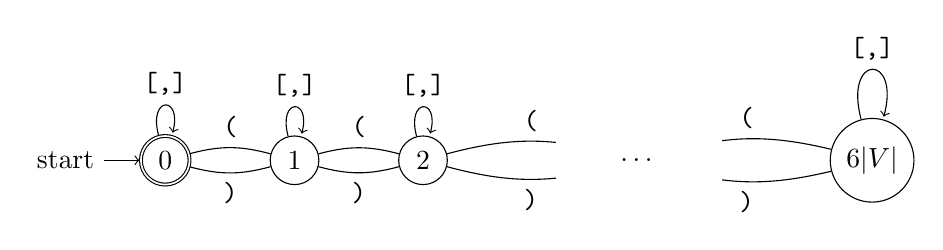
\begin{tikzpicture}
        \node[state, initial, accepting](n0) {$0$};
        \node[state, right=of n0](n1) {$1$};
        \node[state, right=of n1](n2) {$2$};
        \node[state, right=6em of n2](n3) {$3$};
        \node[state, right=6em of n3](n4) {$6|V|$};

        \foreach \y [evaluate=\y as \ny using int(\y+1)] in {0,1} {
          \draw (n\y)  edge[bend left=15] node[above] {\tt (} (n\ny);
          \draw (n\ny) edge[bend left=15] node[below] {\tt )} (n\y);
        }

        \foreach \y [evaluate=\y as \ny using int(\y+1)] in {2,3} {
          \draw (n\y)  edge[bend left=15] node[above] {\tt (} (n\ny);
          \draw (n\ny) edge[bend left=15] node[below] {\tt )} (n\y);
        }


        \foreach \y  in {0,1,2,4} {
          \draw (n\y) edge[loop above] node{\tt [,]} (ny);
        }

        \node [thick, fill=white, shape=rectangle, minimum width=6em, minimum height=4em, anchor=center] at ([yshift=0em]n3) {$\dots$};
      \end{tikzpicture}
      \caption{Автомат для языка $\cool{D}_p^{6|V|}$}
      \label{img:dyck_6n_dfa}
    \end{figure}

    % Строим такие ДКА для обоих типов скобок. Т.к. и тот, и другой регулярный, то можем их прекрасно пересечь с нашим графом. 

    % Получается такой граф троек $(u, b, p)$ (вершина, баланс квадратных скобок, баланс круглых скобок) на $\O(n^3)$ вершинах и $\O(n^2 m)$ рёбрах.

    % Ещё в нём будут $\eps$-рёбра, найденные второй частью алгоритма. Эти рёбра имеют вид $(u, 6|V|, a) \to (v, 6|V|, b)$. Для всех возможных пар $a/b$ и $u/v$ их $\O(n^4)$.

    После этого нужно решить задачу достижимости для полученного графа-автомата. Покажем, что он получается неориентированным: из-за двунаправленности графа ребро $(u, b, p) \to (v, b+1, p)$ существует тогда и только тогда, когда и обратное ему. То же и с $\eps$-рёбрами: если есть путь, с балансом $(0, j-i)$, то есть и путь в обратную сторону с балансом $(0, i-j)$.

    В неориентированном графе выделяем компоненты связности, теперь из вершины $u$ есть $\cool{D}_p \odot \cool{D}_p$-путь, если $(u, 0, 0)$ и $(v, 0, 0)$ лежат в одной компоненте.

    Итого, эта часть алгоритма работает за dfs по графу-произведению, то есть за $\O(|V|^4)$.

    % Т.к. входной граф двунаправленный, то полученное произведение будет неориентированным (\textit{это не совсем тривиально, но понятно}), значит достижимость на нём можно искать просто dfs'ом за $\O(n^4)$.

    \item {\bf Часть пути, лежащая в $\mathbf{[0, 6|V|] \times [6|V| + 1, +\oo)}$}

    % В какой момент пути идут гулять? Когда вложенность одной из скобок ровно $6|V|$. А когда возвращаются? Тоже когда ровно $6|V|$. А во все моменты между $\ge 6|V|$. 

    % То есть хотим искать такие пути, что по одной скобке они просто сбалансированы ($6|V| \path 6|V|$), а по другой какие попало, но всё время не больше $6|V|$ ($a \path b$, $a, b \le 6|V|$). 

    Хотим найти все пути вида $(u, 6|V|, b_1) \path (v, 6|V|, b_2)$, то есть пути, образующие правильные круглые ПСП, а по квадратным дающие разницу балансов $b_2 - b_1$. При этом квадратный баланс не должен подниматься выше $6|V|$ и опускаться ниже 0 (то есть важно его стартовое значение).

    Будем решать отдельно для каждого стартового квадратного баланса $b_1$. Снова делаем это через пересечения языков. Первый~--- входной граф, второй~--- круглые ПСП (язык $\cool{D}_p$ из~\ref{fact:intersection}). Третий~--- регулярный язык, считающий квадратный баланс $\cool{D}_b^{b_1, 6|V|}$, его единственное отличие от языков в прошлом пункте в том, что баланс может опускаться не до 0, а до $-b_1$ (и подниматься до $6|V| - b_1$, а не до $6|V|$).

    Пересекаем языки в хитром порядке: сначала первый и третий (т.е. входной граф и регулярный язык), получим опять-таки граф пар $(v, p)$~--- вершина и круглый баланс~--- на $\O(|V|^2)$ вершинах и $\O(|V||E|)$ рёбрах. Дальше нужно пересечь его со вторым языком, который просто является языком Дика. Заметим, что граф $G \cap \cool{D}_b^{b_1, 6|V|}$~--- двунаправленный (\TODO: картинка про это), а задача Диковой достижимости на двунаправленных графах решается за $\O(|V| \alpha(|V|) + |E|)$ (в нашем случае, получится $\O(|V||E|)$. Решаем её, теперь путь $(u, 6|V|, b_1) \path (v, 6|V|, b_2)$ существует тогда и только тогда, когда $(v, b_2 - b_1)$ диково достижимо из $(u, 0)$ в полученном графе.

    Получаем алгоритм за $\O(|V||E|)$ для каждого $b_1$, итого $\O(|V|^2 |E|)$.


    % Опять-таки, решаем через пересечение языков. Первый~--- наш граф ($L_1$). Второй~--- просто язык Дика ($L_2$) (опять-таки с оговорками про то, что скобочка другого типа~--- это то же, что и $\eps$). Третий~--- пути Дика, начинающиеся в балансе $a$ и заканчивающиеся в балансе $b$ ($L_3$) (решаем для всех возможных пар балансов, чтобы рёбра провести). Давайте решать отдельно для каждого $a$, то есть нам нужен язык Диковых последовательностей со стартовым балансом $a$, таких, что их баланс не уходит в минус. Язык, опять-таки регулярный. 

    % Дальше пересекаем. Сначала пересекаем $L_1 \cap L_2$. Это просто прямое произведение~--- граф пар $(u, b)$ (для каждого $a$ отдельно, снаружи всего это как бы фор по $a$). Вершин в нём $\O(n^2)$, рёбер $\O(n m)$. Теперь нужно это ещё пересечь с $L_3$. Ну так это же просто язык Дика, а Дикову достижимость мы за $\O(m^{*} \alpha)$ на двунаправленных графах решаем (а произведение $L_1 \cap L_2$ как раз двунаправленное). 

    % \TODO: допереписать

    % Получаем $\O(n \cdot n m^{*} \alpha) = \O(n^4 \alpha)$.

\end{enumerate}

\begin{theorem}
  Для задачи $\cool{D}_1 \odot \cool{D}_1$-достижимости существует алгоритм с временем работы $\O(|V|^4)$.
\end{theorem}

\subsection{Выводы и результаты по главе}

\TODO
% \section*{Заключение}


\includegraphics[width=0.75\linewidth]{img/conclusion_goal}

Главным результатом данной работы является новый подход для разработки частный решений для задачи поиска путей с контекстно-свободными ограничениями.

\bibliographystyle{ugost2008ls}
\bibliography{diploma.bib}
\end{document}
